\documentclass[letterpaper]{article}
\usepackage[margin=0.65in,top=0.72in,bottom=0.64in,headheight=15pt,headsep=16pt]{geometry}
\usepackage[T1]{fontenc}
\usepackage{lmodern}
\usepackage{tikz}
\usetikzlibrary{arrows.meta,positioning}
\usepackage{fancyhdr}
\usepackage{xcolor}
\definecolor{redword}{RGB}{218,94,83}
\definecolor{yellowword}{RGB}{247,212,83}
\pagestyle{fancy}
\fancyhf{}
\renewcommand{\headrulewidth}{0.4pt}
\renewcommand{\footrulewidth}{0pt}
\fancyfoot[L]{\footnotesize Bellingham Math Circle / Week 6 / F06-RV-v1}
\fancyfoot[R]{\footnotesize\thepage}
\setlength{\parindent}{0pt}
\setlength{\parskip}{9pt}
\newcommand{\band}[1]{\fancyhead[L]{\small Week 6 / Code breaking / Grades #1}}
\newcommand{\problem}[1]{\textbf{Problem #1:} }
\newcommand{\counter}[3]{\node[draw,fill=#3,circle,minimum size=0.27in,inner sep=0pt,font=\small\bfseries] at (#1,0) {#2};}
\newcommand{\card}[3]{\draw[rounded corners=3pt] (#1,#2) rectangle ++(0.52,0.52);\node[font=\large] at (#1+0.26,#2+0.26) {#3};}
\begin{document}
\fontsize{15.5}{20}\selectfont
\band{2--5}

The keeper secretly chooses one heavy card. Put equal numbers of cards on the two pans. The keeper says LEFT or RIGHT if that pan holds the heavy card, and BALANCED if neither pan does. The secret stays the same.

\begin{center}
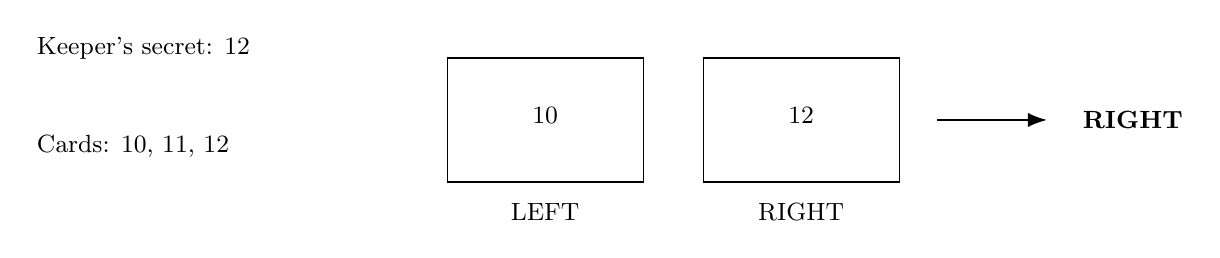
\begin{tikzpicture}[x=1in,y=1in,font=\small]
  \node[anchor=west] at (0,0.77) {Keeper's secret: 12};
  \draw (2.1,0.1) rectangle (3.08,0.72);
  \draw (3.38,0.1) rectangle (4.36,0.72);
  \node at (2.59,0.43) {10};
  \node at (3.87,0.43) {12};
  \node at (2.59,-0.05) {LEFT};
  \node at (3.87,-0.05) {RIGHT};
  \draw[-{Latex[length=7pt]},thick] (4.55,0.41) -- (5.1,0.41);
  \node[anchor=west,font=\small\bfseries] at (5.23,0.41) {RIGHT};
  \node[anchor=west] at (0,0.28) {Cards: 10, 11, 12};
\end{tikzpicture}
\end{center}

\problem{1} Find a weighing plan that always identifies the heavy card among 1--9. What is the fewest weighings you can guarantee, even when the keeper chooses the hardest secret?

\begin{center}
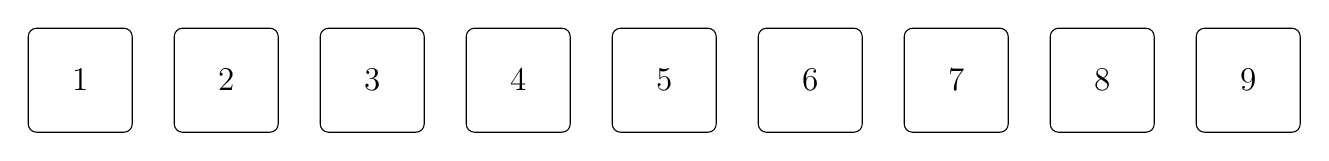
\begin{tikzpicture}[x=1in,y=1in]
  \foreach \n in {1,...,9} {\pgfmathsetmacro{\xx}{(\n-1)*0.73}\card{\xx}{0}{\n}}
\end{tikzpicture}
\end{center}

\begin{center}
\begin{tikzpicture}[x=1in,y=1in,font=\small]
  \draw[line width=1pt] (0,0) rectangle (3.05,1.35);
  \draw[line width=1pt] (3.63,0) rectangle (6.68,1.35);
  \node at (1.525,1.52) {LEFT};
  \node at (5.155,1.52) {RIGHT};
\end{tikzpicture}
\end{center}

\vspace{0.1in}
\begin{center}
\begin{tikzpicture}[x=1in,y=1in]
  \draw[gray!50] (0,0) rectangle (6.68,2.25);
\end{tikzpicture}
\end{center}

\newpage
\band{4--5}

The keeper hides a letter. A yes/no question may ask whether it belongs to any group of letters. Start each message with all four letters possible. Stop as soon as only one letter is possible.

\problem{2} These eight messages will each be sent once. Find a question plan that uses the fewest questions in total across the whole batch. Use the same plan for every message, with later questions allowed to depend on earlier answers. What is the most questions your plan needs for one message?

\begin{center}
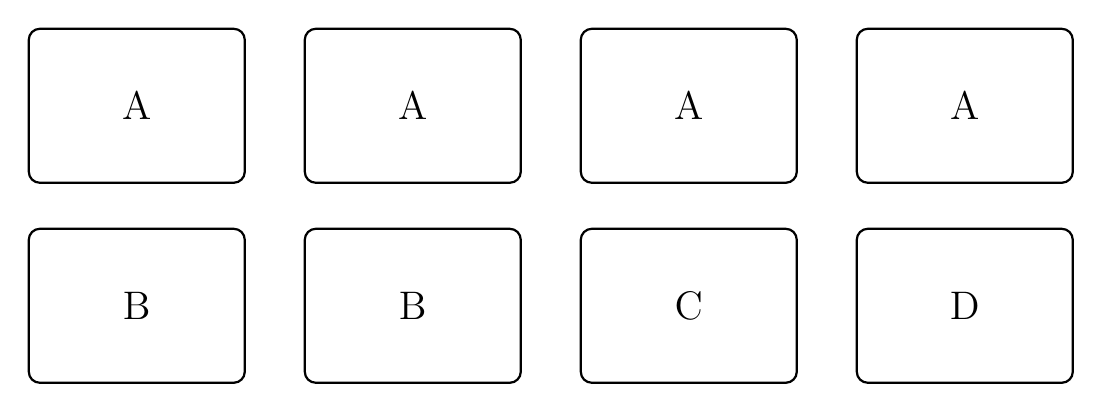
\begin{tikzpicture}[x=1in,y=1in,font=\Large]
  \foreach \x/\y/\t in {0/1.0/A,1.38/1.0/A,2.76/1.0/A,4.14/1.0/A,0/0/B,1.38/0/B,2.76/0/C,4.14/0/D} {
    \draw[rounded corners=4pt,line width=0.8pt] (\x,\y) rectangle ++(1.08,0.77);
    \node at (\x+0.54,\y+0.385) {\t};
  }
\end{tikzpicture}
\end{center}

\vspace{0.15in}
\begin{center}
\begin{tikzpicture}[x=1in,y=1in]
  \draw[gray!50] (0,0) rectangle (6.68,3.02);
\end{tikzpicture}
\end{center}

\vspace{0.05in}
\begin{center}
\begin{tikzpicture}[x=1in,y=1in,font=\small]
  \node[anchor=west] at (0,0.75) {Questions for one message:};
  \foreach \x/\t in {0/A,1.65/B,3.3/C,4.95/D} {
    \node[anchor=west,font=\normalsize] at (\x,0.2) {\t};
    \draw (\x+0.42,0.03) -- (\x+1.25,0.03);
  }
  \node[anchor=west] at (0,-0.55) {Total for the eight messages:};
  \draw (2.6,-0.69) -- (4.18,-0.69);
\end{tikzpicture}
\end{center}

\newpage
\band{2--5}

R is a red counter and Y is a yellow counter. Replace each letter by its counter word, then join the words without spaces.

\begin{center}
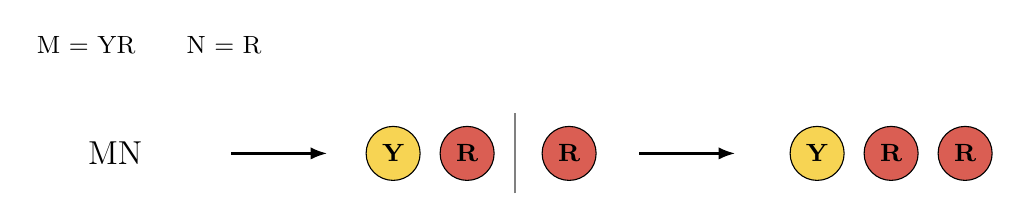
\begin{tikzpicture}[x=1in,y=1in,font=\small]
  \node[anchor=west] at (0,0.54) {M = YR\qquad N = R};
  \node[font=\large] at (0.44,0) {MN};
  \draw[-{Latex[length=6pt]},thick] (1.02,0) -- (1.5,0);
  \begin{scope}[shift={(1.83,0)}]
    \counter{0}{Y}{yellowword}\counter{0.37}{R}{redword}
    \draw[gray,thick] (0.61,-0.2) -- (0.61,0.2);
    \counter{0.88}{R}{redword}
  \end{scope}
  \draw[-{Latex[length=6pt]},thick] (3.06,0) -- (3.54,0);
  \begin{scope}[shift={(3.95,0)}]
    \counter{0}{Y}{yellowword}\counter{0.37}{R}{redword}\counter{0.74}{R}{redword}
  \end{scope}
\end{tikzpicture}
\end{center}

\problem{3} Which books let two different letter messages make exactly the same counter row? Find two such messages, or explain why a sent row can only be read one way. You may use a letter more than once.

\begin{center}
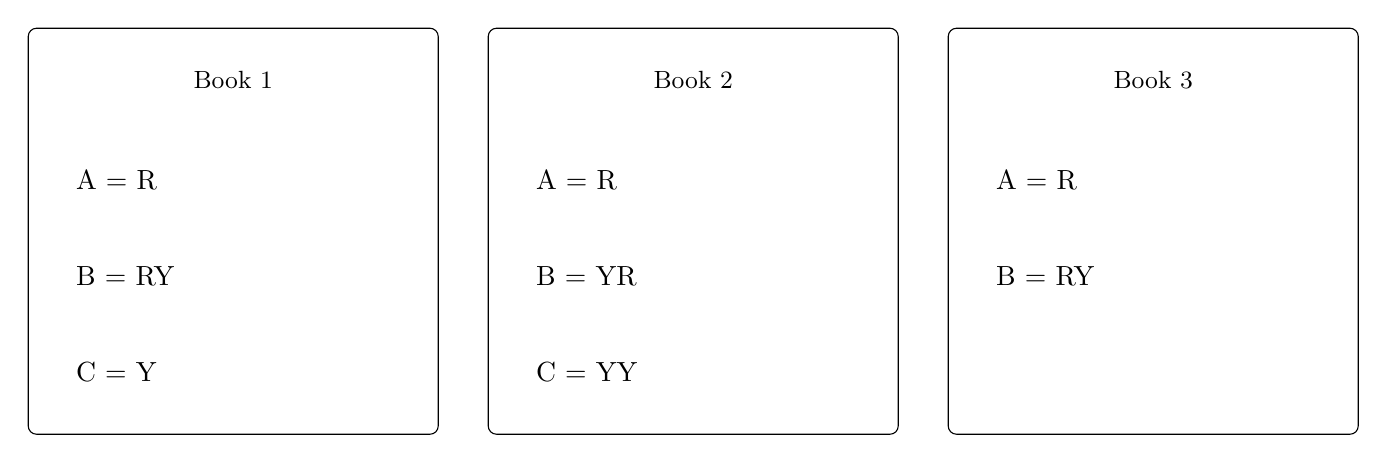
\begin{tikzpicture}[x=1in,y=1in,font=\normalsize]
  \foreach \x/\book in {0/1,2.3/2,4.6/3} {
    \draw[rounded corners=3pt] (\x,-1.52) rectangle (\x+2.05,0.51);
    \node[font=\small] at (\x+1.025,0.25) {Book \book};
  }
  \node[anchor=west] at (0.19,-0.25) {A = R};
  \node[anchor=west] at (0.19,-0.73) {B = RY};
  \node[anchor=west] at (0.19,-1.21) {C = Y};
  \node[anchor=west] at (2.49,-0.25) {A = R};
  \node[anchor=west] at (2.49,-0.73) {B = YR};
  \node[anchor=west] at (2.49,-1.21) {C = YY};
  \node[anchor=west] at (4.79,-0.25) {A = R};
  \node[anchor=west] at (4.79,-0.73) {B = RY};
\end{tikzpicture}
\end{center}

\vspace{0.15in}
\begin{center}
\begin{tikzpicture}[x=1in,y=1in]
  \draw[gray!50] (0,0) rectangle (6.65,3.5);
\end{tikzpicture}
\end{center}

\end{document}
